\documentclass[12pt,letterpaper]{article}
\usepackage{graphicx,textcomp}
\usepackage{natbib}
\usepackage{setspace}
\usepackage{fullpage}
\usepackage{color}
\usepackage[reqno]{amsmath}
\usepackage{amsthm}
\usepackage{fancyvrb}
\usepackage{amssymb,enumerate}
\usepackage[all]{xy}
\usepackage{endnotes}
\usepackage{lscape}
\newtheorem{com}{Comment}
\usepackage{float}
\usepackage{hyperref}
\newtheorem{lem} {Lemma}
\newtheorem{prop}{Proposition}
\newtheorem{thm}{Theorem}
\newtheorem{defn}{Definition}
\newtheorem{cor}{Corollary}
\newtheorem{obs}{Observation}
\usepackage[compact]{titlesec}
\usepackage{dcolumn}
\usepackage{tikz}
\usetikzlibrary{arrows}
\usepackage{multirow}
\usepackage{xcolor}
\newcolumntype{.}{D{.}{.}{-1}}
\newcolumntype{d}[1]{D{.}{.}{#1}}
\definecolor{light-gray}{gray}{0.65}
\usepackage{url}
\usepackage{listings}
\usepackage{color}

\definecolor{codegreen}{rgb}{0,0.6,0}
\definecolor{codegray}{rgb}{0.5,0.5,0.5}
\definecolor{codepurple}{rgb}{0.58,0,0.82}
\definecolor{backcolour}{rgb}{0.95,0.95,0.92}

\lstdefinestyle{mystyle}{
	backgroundcolor=\color{backcolour},   
	commentstyle=\color{codegreen},
	keywordstyle=\color{magenta},
	numberstyle=\tiny\color{codegray},
	stringstyle=\color{codepurple},
	basicstyle=\footnotesize,
	breakatwhitespace=false,         
	breaklines=true,                 
	captionpos=b,                    
	keepspaces=true,                 
	numbers=left,                    
	numbersep=5pt,                  
	showspaces=false,                
	showstringspaces=false,
	showtabs=false,                  
	tabsize=2
}
\lstset{style=mystyle}
\newcommand{\Sref}[1]{Section~\ref{#1}}
\newtheorem{hyp}{Hypothesis}

\title{Problem Set 2: QTM 200: Applied Regression Analysis}
\date{Due: February 10, 2020}
\author{Farris Sabir}

\begin{document}
	\maketitle
	
	\section*{Instructions}
	\begin{itemize}
		\item Please show your work! You may lose points by simply writing in the answer. If the problem requires you to execute commands in \texttt{R}, please include the code you used to get your answers. Please also include the \texttt{.R} file that contains your code. If you are not sure if work needs to be shown for a particular problem, please ask.
		\item Your homework should be submitted electronically on the course GitHub page in \texttt{.pdf} form.
		\item This problem set is due at the beginning of class on Monday, February 10, 2020. No late assignments will be accepted.
		\item Total available points for this homework is 100.
	\end{itemize}
	
	\vspace{.5cm}
	\section*{Question 1 (40 points): Political Science}
		\vspace{.25cm}
	The following table was created using the data from a study run in a major Latin American city.\footnote{Fried, Lagunes, and Venkataramani (2010). ``Corruption and Inequality at the Crossroad: A Multimethod Study of Bribery and Discrimination in Latin America. \textit{Latin American Research Review}. 45 (1): 76-97.} As part of the experimental treatment in the study, one employee of the research team was chosen to make illegal left turns across traffic to draw the attention of the police officers on shift. Two employee drivers were upper class, two were lower class drivers, and the identity of the driver was randomly assigned per encounter. The researchers were interested in whether officers were more or less likely to solicit a bribe from drivers depending on their class (officers use phrases like, ``We can solve this the easy way'' to draw a bribe). The table below shows the resulting data.

\newpage
\begin{table}[h!]
	\centering
	\begin{tabular}{l | c c c }
		& Not Stopped & Bribe requested & Stopped/given warning \\
		\\[-1.8ex] 
		\hline \\[-1.8ex]
		Upper class & 14 & 6 & 7 \\
		Lower class & 7 & 7 & 1 \\
		\hline
	\end{tabular}
\end{table}

\begin{enumerate}
	
	\item [(a)]
	Calculate the $\chi^2$ test statistic by hand (even better if you can do "by hand" in \texttt{R}).\\
	\vspace{.5cm}
	A matrix was first created in R to represent the above table.
	\lstinputlisting[language=R, firstline=40, lastline=41]{PS2.R}  
	\vspace{.5cm}
	Then, a new matrix was filled given expected values derived from the sum of each row in the original matrix and the sume of each column. Each expected value was calculated as the product of the sum of its row's values and the sum of its column's values divided by the total number of observations.
	\lstinputlisting[language=R, firstline=45, lastline=52]{PS2.R} 
	Note: because two of the six expected values are less than 5, a chi-squared test may not be appropriate to draw conclusions about this data, so this should be noted when interpreting the final results.
	\vspace{.5cm}
	Then, the differences between the matrix of observed values and the matrix of expected values were input to another matrix, and that matrix's sum was equivalent to the test statistic, which was 3.79.
	\lstinputlisting[language=R, firstline=55, lastline=56]{PS2.R} 
	\vspace{.5cm}
	
	\item [(b)]
	Now calculate the p-value (in \texttt{R}).\footnote{Remember frequency should be $>$ 5 for all cells, but let's calculate the p-value here anyway.}  What do you conclude if $\alpha = .1$?\\
	
	\vspace{.5cm}
	
	The test-statistic of 3.79 can be used, as well as the degrees of freedom calculated from the number of rows and columns, to provide the p-value. The p-value of 0.1502 is greater than the alpha of 0.1, which leads to failing to reject the null hypothesis that the class of the employee and the response of the police are statistically independent. R's chisq.test function supported this lack of a statistically significant relationship or dependence.
	\lstinputlisting[language=R, firstline=59, lastline=65]{PS2.R} 
	\vspace{.5 cm}
	\item [(c)] Calculate the standardized residuals for each cell and put them in the table below.
	After creating an empty matrix similar to the original one to input the residual values, the standardized residual for each value of the original table was calculated and input. The coding and the eventual table of residuals are shown below: 
	\lstinputlisting[language=R, firstline=68, lastline=80]{PS2.R} 
	\vspace{1cm}
	
	\begin{table}[h]
		\centering
		\begin{tabular}{l | c c c }
			& Not Stopped & Bribe requested & Stopped/given warning \\
			\\[-1.8ex] 
			\hline \\[-1.8ex]
			Upper class  & 0.3220306 & -1.641957 & 1.523026  \\
			\\
			Lower class & -0.3220306 & 1.641957  & -1.523026  \\
			
		\end{tabular}
	\end{table}
	
	
	\vspace{.5cm}
	\item [(d)] How might the standardized residuals help you interpret the results?  
	After the conclusion to fail to reject the null hypothesis that the class of employees and response of police was independent, the relationship between the two variables can be further explored. The test led to failing to reject the null hypothesis, which is consistent with residuals whose absolute values are not very large. The expected and observed values are not greatly different, in other words. The conditions where the employees were not stopped had the least deviation from independence whereas the toher conditions relatively experienced the most. However, the residuals were never different enough from each other to conclude any statistically significant dependence.
	\vspace{.5 cm}
	


	
\end{enumerate}
\newpage

\section*{Question 2 (20 points): Economics}
Chattopadhyay and Duflo were interested in whether women promote different policies than men.\footnote{Chattopadhyay and Duflo. (2004). ``Women as Policy Makers: Evidence from a Randomized Policy Experiment in India. \textit{Econometrica}. 72 (5), 1409-1443.} Answering this question with observational data is pretty difficult due to potential confounding problems (e.g. the districts that choose female politicians are likely to systematically differ in other aspects too). Hence, they exploit a randomized policy experiment in India, where since the mid-1990s, $\frac{1}{3}$ of village council heads have been randomly reserved for women. A subset of the data from West Bengal can be found at the following link: \url{https://raw.githubusercontent.com/kosukeimai/qss/master/PREDICTION/women.csv}\\

\noindent Each observation in the data set represents a village and there are two villages associated with one GP (i.e. a level of government is called "GP"). Figure~\ref{fig:women_desc} below shows the names and descriptions of the variables in the dataset. The authors hypothesize that female politicians are more likely to support policies female voters want. Researchers found that more women complain about the quality of drinking water than men. You need to estimate the effect of the reservation policy on the number of new or repaired drinking water facilities in the villages.
\vspace{.5cm}
\begin{figure}[h!]
	\caption{\footnotesize{Names and description of variables from Chattopadhyay and Duflo (2004).}}
	\vspace{.5cm}
	\centering
	\label{fig:women_desc}
	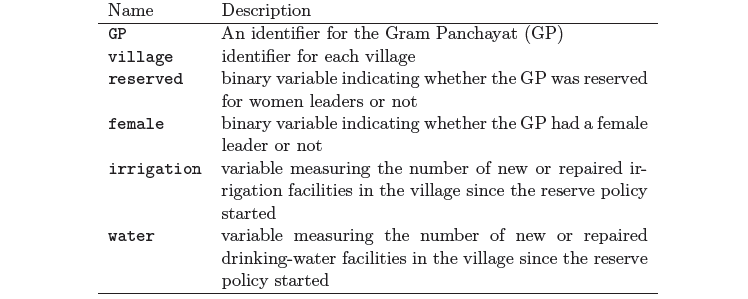
\includegraphics[width=1.1\textwidth]{./women_desc.png}
\end{figure}		

\newpage
\begin{enumerate}
	\item [(a)] State a null and alternative (two-tailed) hypothesis. 
	
	The null hypothesis is that the slope of the linear approximation of the relationship between the average number of new and repaired drinking-water facilities in villages and the number of villages with the reservation policy implemented is equal to zero. Formally, $H_o: \beta_1 = 0 $.
	The alternative hypothesis is that the slope of the linear approximation of the relationship between the average number of new and repaired drinking-water facilities in villages and the number of villages with the reservation policy implemented is unequal to zero. Formally, $H_a: \beta_1 \neq 0 $.
	
	\vspace{.5cm}
	
	\item [(b)] Run a bivariate regression to test this hypothesis in \texttt{R} (include your code!).
	First, the data needed to be input.
	
	\lstinputlisting[language=R, firstline=98, lastline=99]{PS2.R} 
	
	Before conducting the bivariate regression, some assumptions need to be addressed. First, the data must be assumed to have been generated randomly, which is reasonable given the policy was randomly assigned to some villages versus others. Second, the observations have to be assumed to be independent, like one village's choice to change the number of facilities did not influence another's choice. Third, a linear relationship must be assumed between the variables of reservation policy and the number of water-drinking facilities in the villages. Finally, the population values of number of water-drinking facilities at both reserved and non-reserved villages must be assumed to follow a normal distribution with the same standard deviation for both reserved and non-reserved villages. Because the residuals center around zero, which can be shown in Figure 2 below, this last assumption can be reasonably met.
	
	\lstinputlisting[language=R, firstline=105, lastline=106]{PS2.R} 
	\vspace{.5cm}
	
	\begin{figure}[h!]
		\caption{\footnotesize{Density of Residuals}}
		\vspace{.5cm}
		\centering
		\label{fig:density_resid2}
		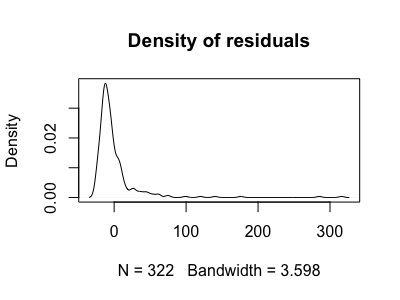
\includegraphics[width=1\textwidth]{./PS2_Graph_1.png}
	\end{figure}	

	In seeking the $\hat{\beta_1} $, the means for the number of villages with the reservation policy and for the number of water-drinking facilities are calculated, and therefrom, $\hat{\beta_1} $ can be found using the equation $\hat{\beta_1} = \frac{\Sigma x_i y_i}{\Sigma x_i^2} $, which produced a $\hat{\beta_1} $ of 9.252.
	\lstinputlisting[language=R, firstline=110, lastline=113]{PS2.R} 
	\vspace{.5cm}	
	
	Meanwhile, the $\hat{\beta_0} $ or $\hat{\alpha} $ is calculated using the mean number of water-drinking facilities, the mean number of villages with the reservation policy, and the $\hat{\beta_1} $, and it proves to be 14.738.
	
	\lstinputlisting[language=R, firstline=117, lastline=118]{PS2.R} 
	\vspace{.5cm}
	
	The null hypothesis is tested for by calculating the standard deviation, standard error of the slope, the t-statistic, and the p-value in that order. Using the standard error, the t-statistic proved to be 2.344, and this helped lead to the resulting p-value of 0.0197. This was verified by R's linear model fitting function.
	
	\lstinputlisting[language=R, firstline=121, lastline=131]{PS2.R} 	
	\vspace{.5cm}
	
	\item [(c)] Interpret the coefficient estimate for reservation policy. 
	\vspace{.5cm}
	
	The coefficient estimate $\hat{\beta_1}$ of 9.252 for the slope is associated with a t-value of 2.344 and p-value of 0.0197, which with an alpha of 0.05, leads to rejecting the null hypothesis. Therefore, the reservation policy led to a significant change in the number of new or repaired drinking-water facilities since the reserve policy started. This can be interpreted so that a 1 unit increase in the number of villages with reservation policy leads to, on average, 9.252 more new or repaired drinking-water facilities. On the other hand, the $\hat{\beta_0}$ or $\hat{\alpha}$ of 14.738 can be interpreted so that, with no reservation policies being implemented in any village, the number of new or repaired drinking-water facilities is approximately 14.738.
	
	\vspace{.5cm}
\end{enumerate}

\newpage
	\section*{Question 3 (40 points): Biology}

There is a physiological cost of reproduction for fruit flies, such that it reduces the lifespan of female fruit flies.  Is there a similar cost to male fruit flies?  This dataset contains observations from five groups of 25 male fruit flies. The experiment tests if increased reproduction reduces longevity for male fruit flies. The five groups are: males forced to live alone, males assigned to live with one or eight newly pregnant females (non-receptive females), and males assigned to live with one or eight virgin females (interested females). The name of the data set is \texttt{fruitfly.csv}.\footnote{Partridge and Farquhar (1981).``Sexual Activity and the Lifespan of Male Fruitflies''. \textit{Nature}. 294, 580-581.}
	\vspace{1cm}

\begin{tabular}{r|l}
	\texttt{No} & serial number (1-25) within each group of 25\\
	\texttt{type} & Type of experimental assignment \\
	& \hspace{0.1in} $1=$ no females  \\
	& \hspace{0.1in} $2=$ 1 newly pregnant female \\
	& \hspace{0.1in} $3=$ 8 newly pregnant females\\
	& \hspace{0.1in} $4=$ 1 virgin female\\
	& \hspace{0.1in} $5=$ 8 virgin females\\
	\texttt{lifespan} & lifespan (days)\\
	\texttt{thorax} & length of thorax (mm)\\
	\texttt{sleep} & percentage of each day spent sleeping\\
\end{tabular}
	\vspace{1cm}
\begin{enumerate}
	
	\item
	Import the data set and obtain summary statistiscs and examine the distribution of the overall lifespan of the fruitflies.  
	
	\lstinputlisting[language=R, firstline=143, lastline=150]{PS2.R} 	
	
	\begin{verbatim}
	       No          type      lifespan         thorax          sleep      
 Min.   : 1   Min.   :1   Min.   :16.00   Min.   :0.640   Min.   : 1.00  
 1st Qu.: 7   1st Qu.:2   1st Qu.:46.00   1st Qu.:0.760   1st Qu.:13.00 
 Median :13   Median :3   Median :58.00   Median :0.840   Median :20.00  
 Mean   :13   Mean   :3   Mean   :57.44   Mean   :0.821   Mean   :23.46  
 3rd Qu.:19   3rd Qu.:4   3rd Qu.:70.00   3rd Qu.:0.880   3rd Qu.:29.00  
 Max.   :25   Max.   :5   Max.   :97.00   Max.   :0.940   Max.   :83.00
	\end{verbatim}
	
	\begin{figure}[h!]
		\caption{\footnotesize{Density of the Lifespans of Fruitflies}}
		\vspace{.5cm}
		\centering
		\label{fig:lifespan}
		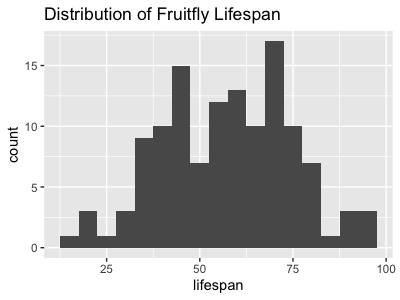
\includegraphics[width=1\textwidth]{./PS2_Graph_2.png}
	\end{figure}	
	
	The data is imported in the above R code and the summary statistics are listed as well. In examining the distribution in Figure 3, the lifespans of fruitflies are approximately normally distributed in this sample.
	
	\vspace{.5cm}

\newpage
	\item
	Plot \texttt{lifespan} vs \texttt{thorax}. Does it look like there is a linear relationship? Provide the plot. What is the correlation coefficient between these two variables?
	
	\vspace{.5cm}
		
	\lstinputlisting[language=R, firstline=153, lastline=154]{PS2.R} 	
	
	\begin{figure}[h!]
	\caption{\footnotesize{Fruitflies' Thorax Length vs. Lifespan}}
	\vspace{.5cm}
	\centering
	\label{fig:lifespanthorax}
	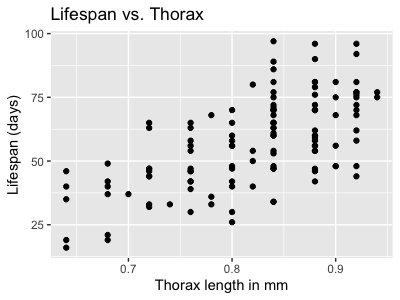
\includegraphics[width=1\textwidth]{./PS2_Graph_3.png}
	\end{figure}

	The above plot in Figure 4 looks as though it shows a linear relationship between thorax length and lifespan.

	\vspace{.5cm}
	
	The correlation coefficient is calculated below using the mean of fruitfly lifespan and mean of fruitfly thorax length as well as their standard deviations. The exact formula is that the coefficient is equal to the covariance between thorax length and lifespan divided by the product of both the standard deviation in thorax length and the standard deviation in lifespan. This proved to be 0.6365 and was verified by R's covariation and correlation functions.

	\lstinputlisting[language=R, firstline=156, lastline=167]{PS2.R} 	
	
	\vspace{.5cm}
	

	\item
	Regress \texttt{lifespan} on \texttt{thorax}.  Interpret the slope of the fitted model.

	\vspace{.5cm}
	
	Before conducting a linear regression, some assumption must be considered. First, the data must be assumed to have been generated randomly, and the types at least were likely randomized. Second, the observations must be assumed to be independent, meaning the thorax length or lifespan of different flies did not influence each other. Third, the relationship between the variables thorax length and lifespan must be assumed to be independent. Finally, the population values of length of thorax at each value of lifespan must be assumed to follow a normal distribution with the same standard deivation for all values of lifespan. This is verified by the residual plot below in Figure 5.
	
	\lstinputlisting[language=R, firstline=174, lastline=175]{PS2.R} 
	
	\begin{figure}[h!]
		\caption{\footnotesize{Density of Residuals}}
		\vspace{.5cm}
		\centering
		\label{fig:density_resid3}
		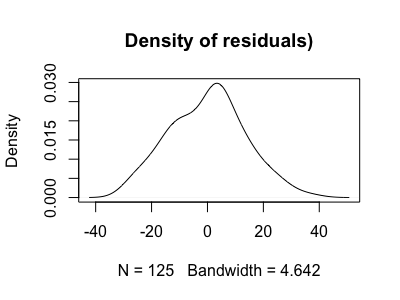
\includegraphics[width=1\textwidth]{./PS2_Graph_4.png}
	\end{figure}	
	
	\vspace{.5cm}
	
	Thereafter, the $\hat{\beta_1}$ can be calculated, using the aforementioned means. This ended up being 144.333. This also helps find $\hat{\beta_0}$ or $\hat{\alpha}$ from the mean lifespan and mean thorax length, and $\hat{\beta_0}$ turned out to be -61.052. These were verified with the R's lienar model fitting function.
	
	\lstinputlisting[language=R, firstline=178, lastline=190]{PS2.R} 
	
	\vspace{.5cm}
	
	The slope of this regression indicates that for every 1 millimeter increase in thorax length, a fruitfly's lifespan is predicted to increase by 144.333 days on average.
	
	
			\vspace{.5cm}
	\item
	Test for a significant linear relationship between  \texttt{lifespan} and \texttt{thorax}. Provide and interpret your results of your test.
	
	\vspace{.5cm}
	
	The null hypothesis is that there is no linear relationship between fruitfly lifespan and thorax length, meaning its correlation coefficient or $\rho = 0$. The alternative hypothesis is that there is a linear relationship between fruitfly lifespan and thorax length, meaning its correlation coefficient of $\rho \neq 0$.
	
	\vspace{.5cm}
	
	To test the null hypothesis that $\rho = 0$, the test statistic was calculated and therefrom, the p-value was calculated. The test statistic using the correlation coefficient that was previously calculated proved to be 9.152 and the p-value proved to be $1.497*10^-15$. This was verified by R's correlation test function.
	
	\lstinputlisting[language=R, firstline=201, lastline=207]{PS2.R} 
	
	\vspace{.5cm}
	
	Because the r value of 0.636 is associated with a t-value of 9.152 and a p-value of $1.497*10^-15$, with an alpha of 0.05, the null hypothesis is rejected. As a result, there is a statistically significant linear relationship between the thorax length and lifespan of fruitflies.
	
	\vspace{1cm}
	
	\item
	
	Provide the 90\% confidence interval for the slope of the fitted model.
	
			\vspace{.5cm}
	\begin{itemize}
		\item
		Use the formula for typical confidence intervals to find the 90\% confidence interval around the point estimate.		\vspace{.5cm}
		\item
		Now, try using the function  \texttt{confint()}  in \texttt{R}.
	\end{itemize}
	
	\vspace{.5cm}
	
	The confidence interval was calculated by finding the t-value that reflects 90\% confidence interval at degrees of freedom of 2, and the margin of error factored in this and the standard error that was calculated from before. The lower and upper limit of the confidence interval was simply the margin of error added to and subtracted from the $\hat{\beta_1}$. The confidence interval proved to be 118 to 170, which was verified by using the function  \texttt{confint()}  in \texttt{R}.
	
	\lstinputlisting[language=R, firstline=214, lastline=224]{PS2.R}

	\vspace{.5cm}
			
	\item Use the \texttt{predict()} function in \texttt{R} to (1) predict an individual fruitfly's lifespan when \texttt{thorax}=0.8 and (2) the average \texttt{lifespan} of fruitflies when \texttt{thorax}=0.8 by the fitted model. This requires that you compute prediction and confidence intervals. What are the expected values of lifespan? What are the prediction and confidence intervals around the expected values? 
	
	\vspace{.5cm}
	
	First, the predict function was used to predict an individual fruitfly's lifespan at thorax of 0.8 mm, which output 54.415 days. The standard error of this prediction was also calculated and proved to be 13.660, and the confidence limits for the predicted value of this lifespan turned out to be 22.268 to 86.562.
	
	\lstinputlisting[language=R, firstline=228, lastline=239]{PS2.R}

	\vspace{.5cm}
	
	Second, the predict function was used to predict the average lifespan of fruitflies when the thorax length is 0.8 by the model, which again output 51.415 days. However, what changed was the standard error of the prediction, which was estimated at 1.261, and the confidence interval, which was calculated at 51.448 to 57.382. 
	
	\lstinputlisting[language=R, firstline=241, lastline=251]{PS2.R}

	
			\vspace{.5cm}
	\item	For a sequence of \texttt{thorax} values, draw a plot with their fitted values for \texttt{lifespan}, as well as the prediction intervals and confidence intervals.
	
	First, a plot for the fitted values for lifespan with prediction intervals given a sequence of thorac values was depicted in Figure 6. A random sample of 20 numbers within the domain of thorax length values was drawn to provide a sequence of thorax values from which the y values or lifespan values could be predicted. This was plotted in a dot plot with the sequence of thorax values against the predicted lifespan values. The standard error and prediction intervals were determined from this and were also taken into account in the plot in the form of error bars.
	
	\lstinputlisting[language=R, firstline=256, lastline=267]{PS2.R}
	
	\begin{figure}[h!]
		\caption{\footnotesize{Sequence of Thorax Values with Fitted Values for Lifespan and Prediction Interval}}
		\vspace{.5cm}
		\centering
		\label{fig:predictionintervals}
		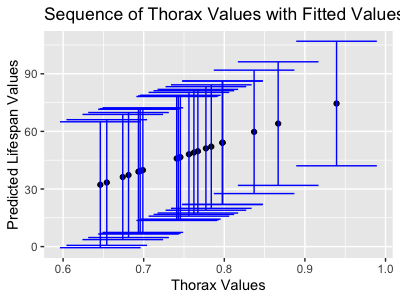
\includegraphics[width=1\textwidth]{./PS2_Graph_5.png}
	\end{figure}	
	
	\vspace{.5cm}
	
	Second, a plot was depicted in Figure 7 for average values of lifespan given a sequence of thorax lengths, the same randomly distributed sample used in the previous step. From this sequence of thorax values, average y values or lifespan values were estimated. This was plotted in a dot plot with the sequence of thorax values against the average lifespan values. The standard error and confidence intervals were determined from this and were also taken into account in the plot in the form of error bars.
	
	\lstinputlisting[language=R, firstline=269, lastline=279]{PS2.R}
	
	\begin{figure}[h!]
		\caption{\footnotesize{Average Lifespan Given Sequence of Thorax Values and Confidence Interval}}
		\vspace{.5cm}
		\centering
		\label{fig:confidenceintervals}
		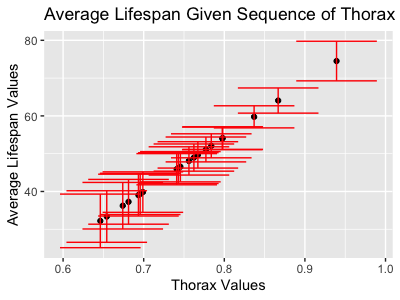
\includegraphics[width=1\textwidth]{./PS2_Graph_6.png}
	\end{figure}	
	
	



\end{enumerate}
\end{document}
